\documentclass[conference]{IEEEtran}

\IEEEoverridecommandlockouts

\usepackage[utf8]{inputenc}
\usepackage{cite}
\usepackage{amsmath,amssymb,amsfonts}
\usepackage{algorithmic}
\usepackage{graphicx}
\usepackage{textcomp}
\usepackage{xcolor}
\usepackage{longtable}

\def\BibTeX{{\rm B\kern-.05em{\sc i\kern-.025em b}\kern-.08em
    T\kern-.1667em\lower.7ex\hbox{E}\kern-.125emX}}
    
\renewcommand{\figurename}{Fig.}
\renewcommand{\tablename}{Tabela}
\renewcommand{\refname}{Referências}

\begin{document}

\title{Mineração de Indicativos de Depressão em Redes Sociais: Um Mapeamento Sistemático}

\author{
    \IEEEauthorblockN{Rodolfo Brandão de Oliveira}
    \IEEEauthorblockA{
    Universidade Tiradentes\\
    Aracaju, Brasil\\
    E-mail: rodolfo.brandao@souunit.com.br
    }
    \and 
    \IEEEauthorblockN{Thiago de Oliveira Lima}
    \IEEEauthorblockA{
    Universidade Tiradentes\\
    Aracaju, Brasil\\
    E-mail: thiago.oliveira@souunit.com.br
    }
}

\maketitle

\begin{abstract}
We live in the information age, where we produce and consume a massive amount of data daily, which directly impacts our lives. One of the most used means for this, and which still has a strong adhesion of new users, are the Social Networks (SN). These can be websites or mobile applications in which a group of people or organizations are able to connect with each other and share subjects on the most diverse topics. We also live in a time when more and more people have developed diseases belonging to the Common Mental Disorders (CMD) group, of which they can manifest themselves in different ways at different ages. One of these evils being depression, this is considered one of the most serious in the CMD group, where there are some studies that associate the use, especially unmoderated, of social networks with the onset or worsening of diseases like this and others of the same group, such as anxiety, especially in the younger community.
\end{abstract}

\begin{IEEEkeywords}
Depressão, Redes Sociais, Artificial Intelligence, Machine Learning, Data Mining, Data Analysis, Clustering Algorithms, Natural Language Processing
\end{IEEEkeywords}

\section{Introdução}
Segundo um dos precursores no campo da realidade virtual e uma das maiores mentes do Vale do Silício, o cientista da computação Jaron Lanier se tornou um grande crítico das redes sociais ao perceber o impacto delas na vida das pessoas. Em seu último livro \cite{JaronLanier}, ele relata que as redes sociais podem atualmente ser consideradas como um segundo documento de identidade e que, além disso, não participar de algumas destas plataformas pode implicar muitas vezes em sinônimo de isolamento total.

No livro, são apresentados 10 argumentos dos quais os indivíduos que já participam de alguma plataforma de mídia social deveriam levar em consideração para abandoná-las. Tais argumentos também se fazem válidos para aqueles que nunca utilizaram nenhuma mídia social. Alguns desses argumentos alegam que as redes sociais tornam as pessoas infelizes, que elas também distorcem a verdade e até mesmo diminuem a capacidade de empatia de seus usuários.

O aumento no uso, na maioria das vezes exacerbado, dessas plataformas tem acarretado no crescimento diretamente proporcional dos casos de depressão entre seus usuários, onde boa parte do problema está associado à maneira na qual essas plataformas são projetadas, com a intenção de prender ao máximo a atenção das pessoas que as utilizam.

Em uma matéria concedida à BBC \cite{BBC}, alguns profissionais do Vale do Silício afirmam que grandes nomes das plataformas de mídias sociais estão deliberadamente levando seus usuários ao vício em seus produtos, visando unicamente o ganho financeiro. Estes afirmam que existem milhares de engenheiros voltados para o design de cada uma das \textit{features} dos produtos dessas companhias, focando seus esforços nos modelos de negócio estabelecidos, dos quais trabalharam ao máximo para torná-las o mais viciante possível.

Com base nesse contexto, identificar meios que possam transparecer aos usuários de redes sociais sobre a situação da saúde mental deles e, consequentemente, demonstrar os perigos que o uso não moderado das mesmas podem acarretar se faz necessário. É importante escalerer à comunidade os riscos que essas plataformas oferecem e que, não bastando isso, a indústria tecnológica não demonstra aparente preocupação para tal fato.

Este trabalho tem como objetivo apresentar um Mapeamento Sistemático da Literatura, o qual visa identificar e transparecer algoritmos, técnicas e abordagens que são utilizados na mineração e detecção de indicativos de possíveis sintomas de depressão em textos (\textit{posts}) advindos exclusivamente de redes sociais. Para tal, artigos pertencentes a área da Ciência da Computação e afins foram pesquisados e mapeados.

Respondendo as questões de pesquisa propostas para este estudo, pôde-se determinar que os principais algoritmos utilizados foram \textit{Clustering} \cite{ArtigoN1, ArtigoN4, ArtigoN5}, Classificação \cite{ArtigoN2, ArtigoN3}, \textit{Deep Learning} \cite{ArtigoN3} e \textit{Supervised Learning} \cite{ArtigoN1, ArtigoN2}. Já a principal abordagem utilizada foi \textit{Natural Language Processing} (NLP) \cite{ArtigoN3, ArtigoN2, ArtigoN4, ArtigoN6, ArtigoN9, ArtigoN10}.

Ocorrências de pesquisas que visam a utilização de redes sociais como meio de extração de informações capazes de demonstrar indicativos de depressão em seus usuários se mostraram recorrentes, uma vez que foi possível identificar um quantidade considerável de trabalhos sobre o tema proposto aqui neste.

Mídias sociais como LiveJournal \cite{ArtigoN11} (7,7\%), Facebook \cite{ArtigoN3, ArtigoN12} (15,4\%), reddit \cite{ArtigoN1, ArtigoN5, ArtigoN6, ArtigoN10} (30,8\%) e Twitter \cite{ArtigoN2, ArtigoN4, ArtigoN7, ArtigoN8, ArtigoN9, ArtigoN12} (46,2\%) foram utilizadas na mineração dos dados levantados nesta pesquisa.

As formas de publicação identificadas mais utilizadas para os trabalhos aqui apresentados se deram em \textit{Proceedings} \cite{ArtigoN1, ArtigoN6, ArtigoN10, ArtigoN12} e \textit{Journals} \cite{ArtigoN2, ArtigoN3, ArtigoN4, ArtigoN5, ArtigoN11}, representando um montante de 33,3\% e 41,6\%, respectivamente. Todas as publicações ocorreram nos anos de 2017 \cite{ArtigoN7, ArtigoN11, ArtigoN12}, 2018 \cite{ArtigoN5}, 2019 \cite{ArtigoN1, ArtigoN3, ArtigoN9, ArtigoN8} e 2020 \cite{ArtigoN2, ArtigoN4, ArtigoN6, ArtigoN10}. Os países com o maior número de trabalhos publicados foram Estados Unidos \cite{ArtigoN2, ArtigoN7, ArtigoN10} com 3 publicações, seguido do México \cite{ArtigoN1, ArtigoN6} com 2.

O restante deste artigo está estruturado da seguinte forma: na seção II são apresentados alguns estudos que evidenciam e sustentam a necessidade do desenvolvimento deste mapeamento sistemático. Na seção III, a metodologia de pesquisa para a execução do mesmo é descrita. Na seção IV são demonstrados os resultados obtidos, realizando uma discussão e análise destes. Por fim, na seção V, são apresentadas algumas ameaças à validade na condução do mapeamento sistemático e em seguida é apresentada a conclusão na seção VI.

\section{Trabalhos Relacionados}
Em um trabalho publicado pela Organização Mundial da Saúde (OMS) \cite{WHO}, estima-se que mais de 300 milhões de pessoas sofrem de depressão ao redor do mundo, cerca de aproximadamente 4,4\% da população global. Existindo também uma parcela aproximada de 3,6\% da massa mundial de pessoas que sofram de transtornos de ansiedade. Sendo regiões como a do Sudeste Asiático e do Pacífico Oriental as mais afetadas. Ainda pode-se constatar o fato de que a predominância nos casos de depressão se dá a indivíduos do sexo feminino em relação aos do sexo oposto.

Condição essa a depressão que é categorizada como um dos Transtornos Mentais Comum (TMC) \cite{CMD} e uma das principais causas de deficiência global, é caracterizada por sintomas como a constante sensação de tristeza, perda de interesse ou prazer, sentimento de culpa, distúrbio no sono ou apetite e até mesmo baixa concentração.

De acordo com um estudo realizado pela Royal Society for Public Health (RSPH) \cite{RSPH}, é relatado que cerca de 91\% das pessoas de 16 à 24 anos utilizam a internet para acessar as redes sociais e que 1 a cada 6 jovens irá experienciar crises de ansiedade em algum momento da vida. Esse mesmo estudo afirma também que as redes sociais são mais viciantes que o álcool e o cigarro e que o índice de depressão entre o grupo de jovens aumentou em cerca de 70\% nos últimos 25 anos.

Essa pesquisa ainda sugere que jovens que fazem uso massivo das redes sociais, gastando mais do que 2 horas diárias, em plataformas como Facebook, Instagram e Twitter, por exemplo, estão mais sujeitos a reportarem uma condição mental precária, incluindo também estresse psicológico (sintomas caracterizados pela ansiedade e depressão).

Mais uma fonte também comprovou tal fato, dessa vez em um experimento no qual foi conduzido pelo prestigiado Journal of the American Medical Association (JAMA) \cite{JAMA}, relatando mais uma vez que, de fato, o uso não moderado das redes sociais aumenta os índices de ansiedade e depressão entre seus usuários. Um grupo de 3826 adolescentes fez parte desse estudo, onde os sintomas de depressão foram medidos utilizando o \textit{Brief Symptoms Inventory} (BSI) \cite{Derogatis}. No trabalho, foi solicitado aos participantes que apontassem, numa escala de 0 (de forma alguma) à 4 (bastante), até que ponto eles experienciaram algum dos 7 sintomas de depressão.

Foi medido também o "tempo de tela" dos participantes ao perguntar quanto tempo eles passam em frente a um computador, celular ou console de \textit{video game}, utilizando redes sociais como o Facebook, Instagram, Twitter ou qualquer outra, jogando, assistindo algum filme ou série, ou outra atividade relacionada. Ainda como parte do experimento, a autoestima de cada um dos participantes também foi medida fazendo uso da escala \textit{Rosenberg Self-Esteem} \cite{Rosenberg}. Ao final, foi possível concluir que o uso exarcebado de eletrônicos como computador e celular, para atividades de lazer como as citadas anteriormente, acarreta no aumento do grau de severidade da depressão para aqueles que já sofram dessa condição. Para indivíduos que não sofram dessa condição, a chance de desenvolver esta mesma se mostrou relativamente alta.

\section{Metodologia}
Para a execução do estudo proposto neste trabalho, um mapeamento sistemático da literatura foi conduzido. Técnica essa que consiste na identificação, avaliação e interpretação de pesquisas disponíveis e relavantes para uma determinada área em particular. A elaboração de um protocolo de pesquisa é também uma tarefa necessária e parte fundamental deste trabalho, baseando-se em 3 aspectos: String de Busca, Questões de Pesquisa e Critérios de Seleção. O protocolo elaborado para tal procedimento se fez baseado nos princípios propostos por Kitchenham \cite{Kitchenham}.

\subsection{Questões de Pesquisa}
O foco deste trabalho consiste na condução de um mapeamento sistemático, visando a identificação de estudos primários que exponham algoritmos, técnicas e abordagens que utilizem processos de mineração de informações que transpareçam possíveis indicativos de sintomas de depressão entre usuários de redes sociais.

Foi baseado nesse contexto que as questões de pesquisa foram elaboradas, objetivando também as métricas utilizadas nos trabalhos pesquisados para estabelecer se determinado texto extraído de uma mídia social é ou não caracterizado por um usuário que possivelmente sofra de depressão. A incidência de pesquisas que fazem uso das redes sociais como fonte de dados para a identificação de depressão também se mostrou um tópico relevante a ser respondido pelo mapeamento sistemático.

Determinar quais destas redes apresentam as maiores incidências nas produção dos trabalhos aqui apresentados se fez também um ponto muito importante a ser esclarecido. Da mesma forma, apontar quais os principais meios de publicação, indicando juntamente o ano de suas publicações e quais os países que tiveram mais trabalhos publicados, também se mostraram tópicos satisfatórios a serem mapeados.

Visando tais questionamentos, as seguintes questões de pesquisa foram elaboradas para a condução do mapeamento sistemático:

\begin{itemize}
    \item \textbf{QP1}: Quais os principais algoritmos, técnicas e abordagens mais utilizadas na identificação de indicativos de depressão em informaçõs extraídas de redes sociais?
    \item \textbf{QP2}: Quais as principais métricas que são levadas em consideração para determinar se um texto possui, ou não, cunho depressivo?
    \item \textbf{QP3}: Qual a incidência de pesquisas que correlacionam temas como redes sociais e detecção de depressão?
    \item \textbf{QP4}: Quais as principais redes sociais utilizadas em trabalhos sobre o tema abordado?
    \item \textbf{QP5}: Quais as principais formas de publicação para trabalhos como os identificados nesta pesquisa?
    \item \textbf{QP6}: Quais foram os anos que houveram mais trabalhos publicados deste gênero?
    \item \textbf{QP7}: Quais os países com mais publicações a respeito do tema apresentado?
\end{itemize}

\subsection{Estratégia de Busca}
Para a realização da pesquisa, a ferramenta de busca para trabalhos científicos Google Acadêmico foi utilizada, na qual uma de suas vantagens consiste na garantia de acesso e uso a qualquer pessoa. Alguns dos artigos que se enquadraram nos critrérios de seleção puderam ser baixados e salvos para posterior tabulação dos seus dados, já outros, porém, por não disponibilizar de acesso para \textit{download}, foram adicionados ao grupo de exclusão do mapeamento.

Através da ocorrência de determinadas palavras-chave, produções acadêmicas foram pesquisadas. Ao final, um apanhado de artigos, em língua inglesa, foram selecionados, sendos estes pertencentes a área da Ciência da Computação e afins (como a bioinformática, por exemplo).

Para tal procedimento, uma string de busca foi formulada utilizando termos que reflitam a necessidade deste trabalho, tendo sido construída da seguinte forma: \textbf{(("depression") AND ("social media") AND ("artificial intelligence" OR "machine learning" OR “data mining” OR “data analysis”) AND ("clustering algorithm") AND ("natural language processing" OR “nlp”))}.

Como resultado da aplicação da string de busca, um total de 274 ocorrências de trabalhos foram retornadas. Após isso, foi dado início na etapa seleção, a qual será detalhada em seguida.

\subsection{Critérios de Seleção}
A fim de manter a integridade da seleção dos trabalhos pesquisados, critérios de inclusão e exclusão foram formulados. A pesquisa utilizou dos seguintes critérios de inclusão para fazer a seleção dos trabalhos:

\begin{itemize}
    \item Os resultados devem conter o tema de estudo no título, \textit{abstract} ou nas palavras-chave;
    \item Os resultados devem discorrer sobre processos de extração e detecção de informações que transpareçam indicativos de depressão em textos advindos exclusivamente de redes sociais;
    \item O ano de publicação dos resultados deve estar contido no intervalo de 2016 à 2020.
\end{itemize}

Para assegurar a relevância dos critérios relatados, a introdução de cada artigo também foi analisada. Da mesma forma, os trabalhos foram validados baseados também nos critérios de exclusão. Estes foram formulados da seguinte forma:

\begin{itemize}
    \item Artigos que não pertencem à área da Ciência da Computação ou afins;
    \item Artigos cujo os trabalhos são secundários;
    \item Artigos com pesquisas em andamento, sem resultados conclusivos;
    \item Artigos sem disponibilidade para \textit{download}.
\end{itemize}

\begin{figure}[h]
    \centering
    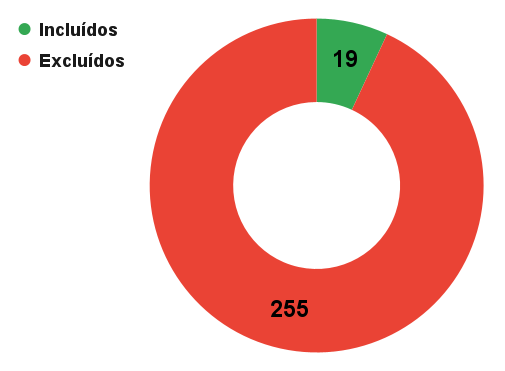
\includegraphics[scale=0.4]{images/quantitativo-trabalhos-avaliados.png}
    \caption{Quantitativo dos trabalhos avaliados}
    \label{fig:quantitativo-trabalhos-avaliados}
\end{figure}

No gráfico da Figura 1 é possível perceber o resultado da aplicação dos critérios de seleção nos resultados obtidos. Dentre o total dos 274 trabalhos retornados como resultado da string de busca, apenas 19 destes se qualificaram nos critérios de seleção e foram adicionados ao grupo de inclusão.

\begin{figure}[h]
    \centering
    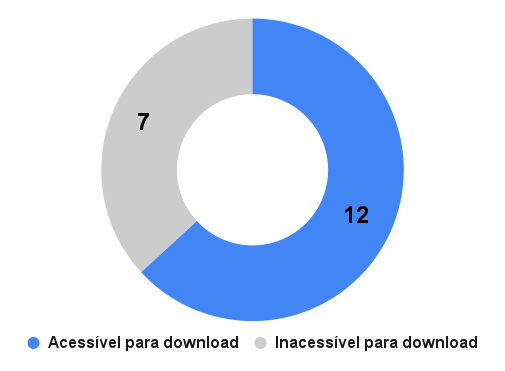
\includegraphics[scale=0.4]{images/acessibilidade-trabalhos-incluidos.png}
    \caption{Acessibilidade dos trabalhos incluídos}
    \label{fig:acessibilidade-trabalhos-incluidos}
\end{figure}

Contudo, como demonstrado na Figura 2, somente uma parcela de 12 trabalhos do grupo de inclusão puderam ter seus dados completamente analisados e mapeados, os demais 7, apesar de expor o título, \textit{abstract}, palavras-chave e introdução, não dispolibilizavam acesso para \textit{download}, o que inviabilizou a leitura de forma completa, acarretando na adição destes ao grupo de exclusão.

\section{Análise dos Resultados}
Nesta seção são discutidos os resultados alcançados após a aplicação da metodologia estabelecida para o mapeamento sistemático, visando expor os dados obtidos e responder a cada uma das questões de pesquisa mencionadas anteriormente.

\begin{figure}[h]
    \centering
    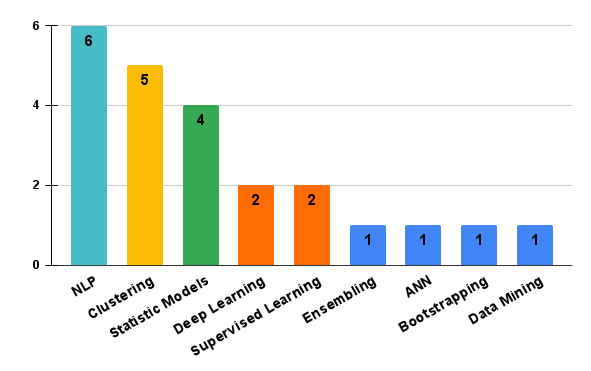
\includegraphics[scale=0.4]{images/abordagens-utilizadas.png}
    \caption{Abordagens utilizadas}
    \label{fig:abordagens-utilizadas}
\end{figure}

O gráfico exibido na Figura 3 expõe as abordagens utilizadas identificadas para a \textbf{QP1}. Sendo as mais relevantes \textit{Natural Language Processing} (NLP) \cite{ArtigoN3, ArtigoN2, ArtigoN4, ArtigoN6, ArtigoN9, ArtigoN10} com 6 incidências, seguido da aplicação algoritmos de Clusterização \cite{ArtigoN1, ArtigoN2, ArtigoN3, ArtigoN4, ArtigoN5} com 5 referências, acompanhado de modelos estatísticos isolados \cite{ArtigoN1, ArtigoN11} com 4 citações. Abordagens que utilizam \textit{Deep Learning} \cite{ArtigoN3} e \textit{Supervised Learning} \cite{ArtigoN1, ArtigoN2} também foram mencionados, com 2 instâncias cada. Por fim, representando 1 única incidência, algoritmo de Conjunto (\textit{ensembling}), \textit{Artificial Neural Network} \cite{ArtigoN8}, \textit{Bootstrapping} \cite{ArtigoN2} e \textit{Data Mining} \cite{ArtigoN8} também foram identificados.

NLP se mostrou a abordagem mais utilizada, demonstrando alta eficiência nos trabalhos pesquisados. Esta é uma subárea da Ciência da Computação e da Linguística, na qual o foco do estudo se baseia na criação de modelos computacionais que utilizam de linguagem humana (natural), possuindo 3 aspectos principais: fonologia, estrutura e significado.

Sua influência nos trabalhos utilizados neste mapeamento sistemático se deu pelo fato de ser uma abordagem capaz de ser aplicada nos textos extraídos das redes sociais visando tratar as informações coletadas, passando inicialmente por uma análise léxica, da qual converte os dados em lexemas (palavra ou parte de uma palavra que serve de base ao sentido por ela expresso). Em seguida é aplicada uma análise sintática, com o objetivo de verificar a gramática, a fim de determinar a relação entre as palavras nela contidas. A informação extraída é também submetida a uma análise semântica, a qual objetiva determinar o significado de cada palavra em um determinado grupo.

Algoritmos de clusterização também se mostraram uma peça fundamental no apanhado dos estudos identificados. Esses algoritmos se caracterizam por ser uma técnica de \textit{machine learning}, na qual se baseia no agrupamento e cálculo da distância entre objetos de um conjunto de dados. Uma vez fornecido um certo conjunto de informações, a técnica de clusterização é capaz de separar esse conjunto em grupos específicos que, em tese, devem ter propriedades similares aos que pertencem a um mesmo grupo, ao mesmo tempo que informações com propriedades distintas devem pertencer a grupos distintos. Dependendo ainda da "direção" dos algoritmos, este poderá ser classificado como \textit{aglomerativo} ou \textit{divisivo}, o que basicamente é a ocorrência da junção ou separação de informações no conjunto de dados.

Ambas as abordagens desempenharam um papel muito importante e eficiente na identificação e rotulação de informações que representem sentimentos negativos e que possam indicar possíveis cenários de depressão.

Alguns recursos também foram identificados nos trabalhos selecionados, como os demonstrados na Tabela 1. O NLTK (\textit{Natural Language Toolkit}) e o scikit-learn, com 3 referências cada, lideram esse grupo.

\begin{table}[h]
    \centering
    \caption{Recursos Utilizados}
    \begin{tabular}[t]{c|c|c}
         \hline
         \textbf{Nome} & \textbf{Incidência} & \textbf{Referência}\\
         \hline
         NLTK & 21,4\% & \cite{ArtigoN2, ArtigoN4, ArtigoN9} \\
         scikit-learn & 21,4\% & \cite{ArtigoN5, ArtigoN7, ArtigoN8} \\
         Word2Vec & 14,3\% & \cite{ArtigoN3, ArtigoN5} \\
         LIWC & 14,3\% & \cite{ArtigoN11, ArtigoN12} \\
         Beautiful Soup & 7,1\% & \cite{ArtigoN4} \\
         fastText & 7,1\% & \cite{ArtigoN6} \\
         Tweepy & 7,1\% & \cite{ArtigoN8} \\
         TextBlob & 7,1\% & \cite{ArtigoN9}
    \end{tabular}
    \label{tab:recursos_utilizados}
\end{table}

Este primeiro é frequentemente utilizado no campo da linguagem natural, na implementação de programas em Python, que auxiliam no processamento da mesma, apresentando \textit{features} como tokenização, lematização, marcação gramatical, segmentação de tópicos, entre outras, o que se faz muito importante na aplicação de NLP nos estudos aqui citados.

Já a segunda menção é conhecida por se tratar de um popular conjunto de ferramentas para análise e predição de dados, sendo baseada nos módulos NumPy, SciPy, e matplotlib, pertencentes também à linguagem de programação Python, além do fato de ser open source.

Outras duas ferramentas representativas foram o Word2Vec e LIWC, com 2 incidências cada. Sendo o Word2Vec a aplicação de uma técnica que utiliza de rede neural para aprender associações de palavras dado um grande volume de texto. Já o LIWC é uma solução paga, sendo uma de suas finalidades calcular o grau de utilização de várias palavras em um conjunto de textos.

Ainda mantendo o foco na \textbf{QP1}, foi possível identificar os principais algoritmos utilizados em cada um dos trabalho selecionados. Sendo o principal e possuindo a maior adesão, baseado no Teorema de Bayes, o algoritmo de classificação Naive Bayes representa uma parcela presente em 17,6\% dos trabalhos mapeados. Este é comumente utilizado em aplicações que envolvam NLP, visando fornecer ocorrências de probabilidades condicionais, ou seja, determinar a probabilidade do evento "A" ocorrer, dado o evento "B". Outro fato é que ele é comumente utilizado para a predição de diagnósticos médicos. Percebemos sua incidência nos trabalhos, assim como a dos demais algoritmos, a partir da Tabela II:

\begin{table}[h]
    \centering
    \caption{Algoritmos Identificados}
    \begin{tabular}[t]{c|c|c}
         \hline
         \textbf{Nome} & \textbf{Incidência} & \textbf{Referência} \\
         \hline
         Naive Bayes & 17,6\% & \cite{ArtigoN2, ArtigoN9, ArtigoN12} \\
         K-means & 11,8\% & \cite{ArtigoN5, ArtigoN7} \\
         Random Forest & 11,8\% & \cite{ArtigoN8, ArtigoN12} \\
         Logistic Regression & 11,8\% & \cite{ArtigoN2, ArtigoN12} \\
         Basilisk & 5,9\% & \cite{ArtigoN2} \\
         Embedding algorithm & 5,9\% & \cite{ArtigoN3} \\
         Modified fuzzy c-means & 5,9\% & \cite{ArtigoN4} \\
         AP & 5,9\% & \cite{ArtigoN1} \\
         LSTM & 5,9\% & \cite{ArtigoN3} \\
         RNN & 5,9\% & \cite{ArtigoN4} \\
         SVM & 5,9\% & \cite{ArtigoN1} \\
         MLP & 5,9\% & \cite{ArtigoN8}
    \end{tabular}
    \label{tab:algoritmos_tecnicas}
\end{table}

O Naive Bayes serviu de grande importância nos artigos pesquisados, uma vez que ajudou os pesquisadores a identificarem indícios de usuários depressivos, baseando-se em uma análise prévia de \textit{posts} advindos dos mesmos, para determinar se a semântica dos textos indicavam sentimentos negativos em relação a saúde mental deles. Em seguida, com 2 ocorrências cada, vêm os algoritmos K-means, \textit{Random Forest} e \textit{Logistic Regression}, representando cerca de 11,8\% nos trabalhos selecionados.

Sendo o primeiro uma técnica de aprendizado não supervisionada, ou seja, que lida com informações não rotuladas. Seu objetivo é identificar similaridades entre os dados fornecidos e tentar agrupá-los conforme o número de \textit{clusters} referenciado no argumento \textit{k}. É um método relativamente simples e eficiente, baseado também no conceito de distância de objetos.

Já o \textit{Random Forest} se baseia na ideia de construção de árvores de decisão para executar a classificação dos dados desejados. Sendo delegada a essas árvores a função de estabelecer as regras de tomada de decisão.

E por último mas não menos importante para os trabalhos avaliados, o algoritmo \textit{Logistic Regression} parte da premissa estatística da construção de um modelo capaz de prover predições através de valores, frequentemente, binários.

Respondendo a \textbf{QP2}, a principal métrica adotada nas pesquisas mapeadas para determinar se as informações extraídas são, ou não, de cunho depressivo, foi a classificação e agrupamento de palavras baseado no sentimento delas, estando presente em 100\% dos trabalhos selecionados. Uma vez escolhidas algumas palavras que indicassem sentimentos como tristeza, baixa autoestima, angústia, rejeição, insatisfação, etc, utilizar essas informações rotuladas na aplicação de modelos que objetivassem indicídios de depressão se tornara um trabalho mais fácil e com maior chance de obtenção de uma boa acurácia. 

É possível transparecer a incidência de pesquisas indicada pela \textbf{QP3} dado os resultados evidenciados na Figura 1. Com a utilização da string de busca foi possível obter uma quantidade considerável de trabalhos dos quais correlacionam redes sociais e depressão para investigar possíveis casos entre seus usuários. Apesar da maioria dos trabalhos não ter se adequado aos critérios de inclusão, uma grande parcela destes revelou altos índices de interesse no tema aqui proposto, sendo boa parte desses trabalhos pertencentes a áreas da medicina, assim como da psicologia.

A evidência das redes sociais utilizadas nos trabalhos abordados se faz através do gráfico apresentado na Figura 4. No qual, para responder a \textbf{QP4}, podemos destacar como as redes sociais mais utilizadas o Twitter \cite{ArtigoN2, ArtigoN4, ArtigoN7, ArtigoN8, ArtigoN9, ArtigoN12}, com 5 incidências (46,2\%), e o reddit \cite{ArtigoN1, ArtigoN5, ArtigoN6, ArtigoN10}, com 4 (30,8\%). Tais plataformas se mostraram as favoritas dos pesquisadores quando o quesito é a extração de dados pois estas disponibilizam de APIs que facilitam essa etapa, assim como \textit{wrappers} (como por exemplo o Tweepy \cite{ArtigoN8}), escritos em Python, que viabilizam o acesso às APIs.

\begin{figure}[h]
    \centering
    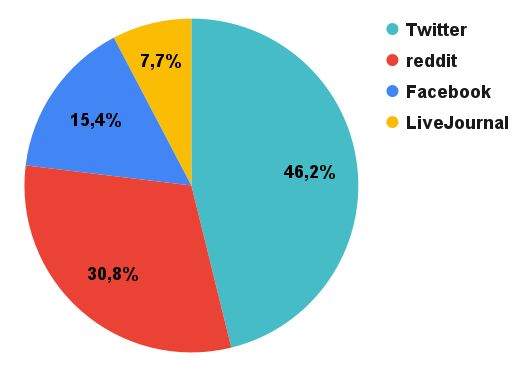
\includegraphics[scale=0.4]{images/redes-sociais-utilizadas.png}
    \caption{Redes sociais utilizadas}
    \label{fig:redes-sociais-utilizadas}
\end{figure}

No que diz respeito à \textbf{QP5}, podemos inferir por meio da Figura 5 que os principais meios de publicação identificados nos trabalhos apresentados na pesquisa deste mapeamento foram \textbf{Journals} \cite{ArtigoN2, ArtigoN3, ArtigoN4, ArtigoN5, ArtigoN11}, com 41,67\%, agregando 5 trabalhos e \textbf{Proceedings} \cite{ArtigoN1, ArtigoN6, ArtigoN10, ArtigoN12}, com 33,33\%, contabilizando 4 publicações. Também foram identificadas produções veiculadas por universidades \cite{ArtigoN7, ArtigoN8, ArtigoN9}, represando uma parcela de 25\%, quantificando um total de 3 trabalhos.

\begin{figure}[h]
    \centering
    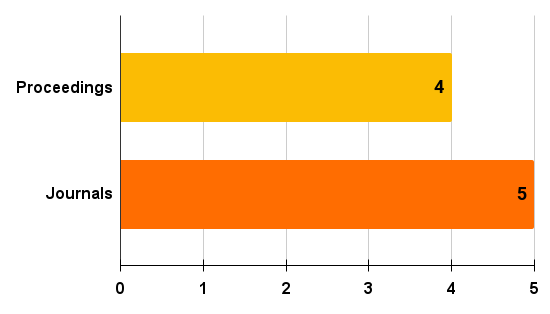
\includegraphics[scale=0.4]{images/distribuicao-journals-proceedings.png}
    \caption{Distribuição dos Journals e Proceedings}
    \label{fig:distribuicao-journals-proceedings}
\end{figure}

No mais, como é demonstrado na Tabela 3, temos os veículos de publicação propriamente ditos para cada uma das referências dos trabalhos pesquisados, sendo esses distintos para cada publicação.

\begin{table}[h]
    \centering
    \caption{Veículos de Publicação}
    \begin{tabular}[t]{c|c}
         \hline
         \textbf{Veículo} & \textbf{Referência} \\
         \hline
         NAACL-HLT & \cite{ArtigoN1} \\
         IJERPH & \cite{ArtigoN2} \\
         IJACSA & \cite{ArtigoN3} \\
         Computers in Human Behavior Reports & \cite{ArtigoN4} \\
         BMC Bioinformatics & \cite{ArtigoN5} \\
         INAOE-CIMAT & \cite{ArtigoN6} \\
         \textit{RIT} & \cite{ArtigoN7} \\
         \textit{UnB} & \cite{ArtigoN8} \\
         \textit{DSpace-UMBM} & \cite{ArtigoN9} \\
         ACL & \cite{ArtigoN10} \\
         JDSA & \cite{ArtigoN11} \\
         ACM & \cite{ArtigoN12}
    \end{tabular}
    \label{tab:veiculos_publicacoes}
\end{table}

Respondendo a \textbf{QP6}, os anos que mais tiveram publicações foram os de 2020 \cite{ArtigoN2, ArtigoN4, ArtigoN6, ArtigoN10} juntamente com o de 2019 \cite{ArtigoN1, ArtigoN3, ArtigoN7, ArtigoN8}. Também foram identificadas publicações para os anos de 2018 \cite{ArtigoN5} e 2017 \cite{ArtigoN9, ArtigoN11, ArtigoN12}, como é demonstrado na Figura 6:

\begin{figure}[h]
    \centering
    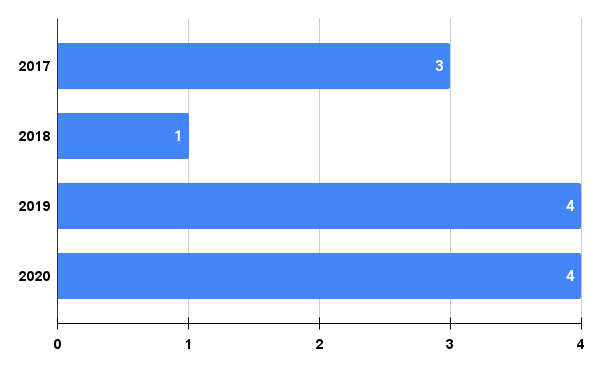
\includegraphics[scale=0.4]{images/quantitativo-publicacoes-por-ano.png}
    \caption{Publicações por ano}
    \label{fig:quantitativo-publicacoes-por-ano}
\end{figure}

Por fim, para a \textbf{QP7}, como ilustrado no gráfico da Figura 7, percebemos os países onde os trabalhos avaliados foram publicados: 

\begin{figure}[h]
    \centering
    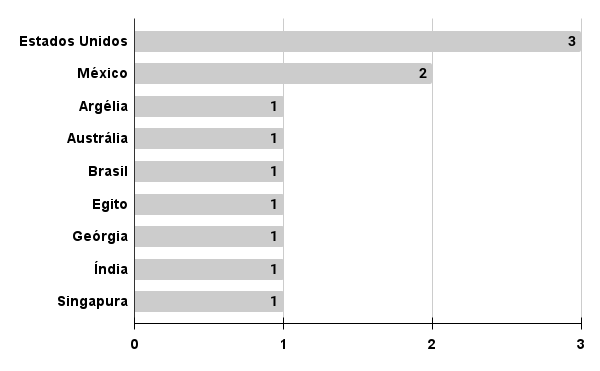
\includegraphics[scale=0.39]{images/quantitativo-publicacoes-por-pais.png}
    \caption{Publicações por país}
    \label{fig:quantitativo-publicacoes-por-pais}
\end{figure}

Ficando evidente que os Estados Unidos \cite{ArtigoN2, ArtigoN7, ArtigoN10} (25\%) e México \cite{ArtigoN1, ArtigoN6} (16,67\%) foram os países que contaram com mais publicações.

Fazendo ainda uma análise mais detalhada sobre os resultados obtidos, por meio da Figura 10 é possível perceber o ano de publicação dos trabalhos para cada um dos seus respectivos países:

\begin{figure}[h]
    \centering
    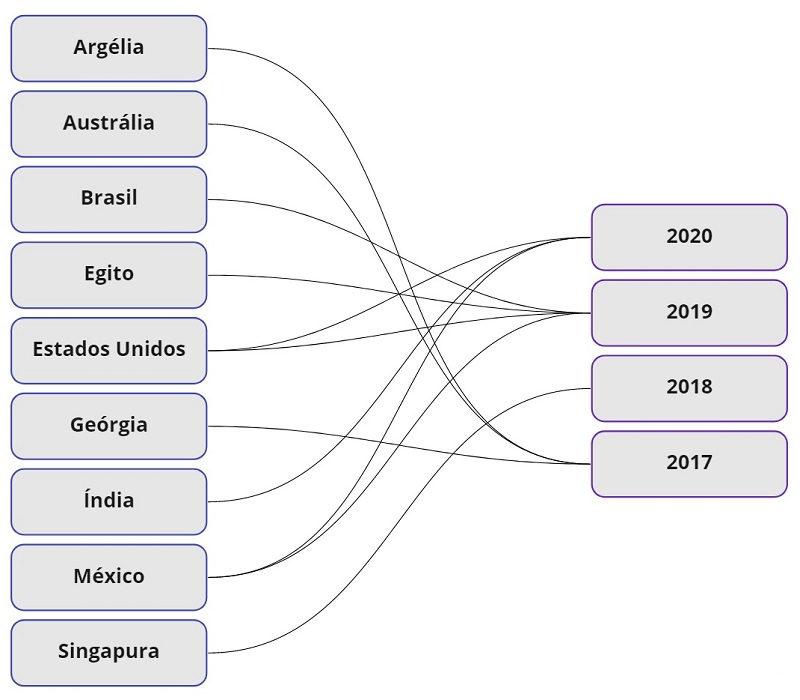
\includegraphics[scale=0.4]{images/ano-publicacao-paises.jpg}
    \caption{Ano das publicações por país}
    \label{fig:ano-publicacao-paises}
\end{figure}

Já como demonstrado pela Figura 9, dessa vez sobre a distribuição dos \textit{Journals} e \textit{Proceedings} ao longo dos anos, sobre todos os trabalhos aqui apresentados, podemos notar o montante de pesquisas veiculadas para cada um dos modelos relatados.

\begin{figure}[h]
    \centering
    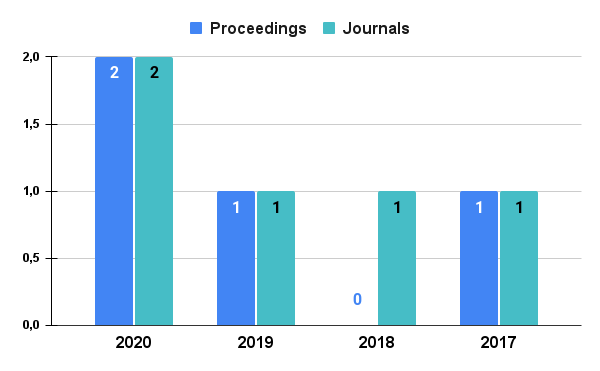
\includegraphics[scale=0.4]{images/quantitativo-tipo-publicacoes-por-ano.png}
    \caption{Distribuição dos Journals e Proceedings por ano}
    \label{fig:quantitativo-tipo-publicacoes-por-ano}
\end{figure}

Exibido pela Figura 10, fica claro perceber ao longo dos anos a utilização do Twitter e reddit, redes sociais mais identificadas como as mais utilizadas na condução dos trabalhos referenciados, sendo possível notar uma maior incidência nos anos de 2020 e 2019 para ambas as plataformas.

\begin{figure}[h]
    \centering
    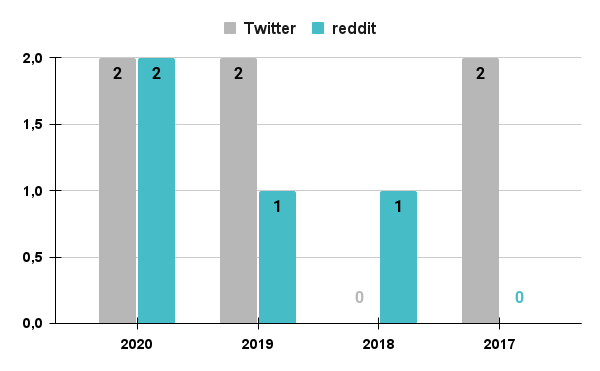
\includegraphics[scale=0.4]{images/redes-sociais-por-ano.png}
    \caption{Utilização do Twitter e o reddit ao longo dos anos}
    \label{fig:redes-sociais-por-ano}
\end{figure}

Finalmente, segundo a Figura 11, é demonstrada a distibuição da escolha de cada mídia social para cada um dos países identificados neste trabalho:

\begin{figure}[h]
    \centering
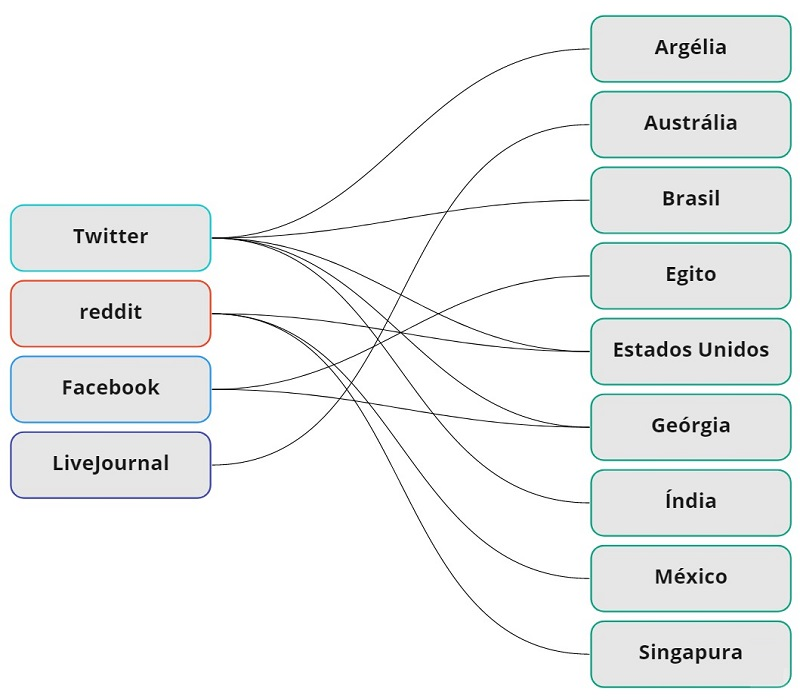
\includegraphics[scale=0.4]{images/redes-sociais-por-pais.jpg}
    \caption{Redes sociais utilizadas por cada país}
    \label{fig:redes-sociais-por-pais}
\end{figure}

\section{Ameaças à Validade}
\textbf{Validade de Construção}: A string de busca elaborada para a condução da pesquisa foi baseada em termos que reflitam a necessidade e a realidade deste trabalho, tendo sido construída da maneira mais abrangente possível, visando viabilizar o resultado de trabalhos que atendam aos interesses deste. Contudo, se faz necessário ressaltar que há a possibilidade da string de busca não ser capaz de abranger toda a área da Ciência da Computação, uma vez que o tema de estudo apresentou grande relevância para outras áreas, como a da saúde, por exemplo.

\textbf{Validade Interna}: \textit{Extração de Dados} - a tabulação dos resultados foi feita de forma manual, examinando cada um dos artigos que se adequaram nos critérios de seleção. Dessa forma, existe probabilidade da ocorrência de problemas ou confusões que possam colocar em xeque a validade desta etapa. 

\textit{Tendência de Seleção} - É importante ressaltar também que algumas publicações podem ter sido categorizadas de forma incorreta, dado o julgamento do grupo de pesquisa, baseado nos critérios de seleção.

\textbf{Validade Externa}: O Google Acadêmico, apesar de ser uma ferramenta de busca amplamente conhecida e que oferece um design familiar e de fácil utilização, apresenta uma grande gama de cobertura de fontes de dados, mas não é abrangente, não sendo recomendada como a única ferramenta a ser utilizada. Também não fornece aos usuários resultados categorizados por disciplina ou área de estudo e uma opção de pesquisa avançada mais refinada.

\section{Conclusão}
Um mapeamento sistemático da literatura foi conduzido neste trabalho, visando identificar as principais produções relacionadas na extração e identificação de indicativos de sintomas de depressão entre usuários de redes sociais, com intuito de determinar as principais tendências no âmbito da Ciência da Computação. Este mapeamento foi executado seguindo as premissas estabelecidas no protocolo de pesquisa apresentado na seção III. Com isso, informações puderam ser extraídas e analisadas a partir de 12 trabalhos distintos, validando as tendências relatadas.

Pôde-se concluir que as abordagens mais relevantes identificadas foram NLP (26,1\%) e Clusterização (21,7\%), da mesma forma que os algoritmos Naive Bayes (17,6\%), K-means, \textit{Random Forest} e \textit{Logistic Regression} (11,8\%) foram os mais utilizados (\textbf{QP1}).

Concentrar o foco na rotulação de textos e/ou palavras que indiquem sentimentos que reflitam a realidade da depressão mostrou-se a mais viável métrica no desenvolvimento dos trabalhos aqui mapeados (\textbf{QP2}).

Foi possível ainda notar que a incidência de pesquisas que correlacionam temas como depressão e a utilização de redes sociais, aparenta ser um tópico promissor entre a comunidade acadêmica da Ciência da Computação em conjunto com a da saúde (\textbf{QP3}).

Redes sociais como Twitter (46,2\%) e reddit (30,8\%) demonstraram ser as favoritas a partir do ponto de vista dos pesquisadores diante da facilidade da extração e manipulação de dados, além de serem amplamente utilizadas em todo o mundo e por disponibilizarem de APIs e \textit{wrappers} que auxiliam nessa etapa (\textbf{QP4}).

Finalmente, para trabalhos como os analisados neste mapeamento sistemático, as principais formas de publicações ocorreram em \textit{Journals} (41,67\%) e \textit{Proceedings} (33,33\%), contando com uma variedade singular de veículos de publicação para cada destes (\textbf{QP5}). Também pôde-se constatar que os anos com mais publicações foram os de 2020 (33,3\%) e 2019 (33,3\%) (\textbf{QP6}). Para os países com mais trabalhos publicados, foram identificados os Estados Unidos (25\%) e México (16,67\%) (\textbf{QP7}).

O tema de estudo abordado neste mapeamento sistemático se mostrou um tópico de suma relevância para a Ciência da Computação, podendo ser mesclado com outras áreas, como a medicina ou a psicologia, para a produção de linhas de pesquisas mais aprofundadas no tema, demonstrando ser, dessa forma, um tema com fortes tendências na comunidade acadêmica. Este trabalho ainda pode servir como base para o desenvolvimento de trabalhos futuros, principalmente para aqueles dos quais a pesquisa tenha como objetivo o tema abordado neste mapeamento.

\bibliography{references}
\bibliographystyle{IEEETran}

\end{document}
